\documentclass[../../main.tex]{subfiles}
\begin{document}

\subsection*{2.5}
Una carica positiva q distante $d = 40\ cm$ da un piano indefinito carico con densità $\sigma = 8,86 * 10^{10}\ \frac{C}{m^2}$.
Un dipolo elettrico di momento $p = 10^{12}\ Cm$, parallelo e concorde al vettore OA equidistante  dal piano è soggetta a $F=2.25 * 10^{-9}\ N$.
\\Calcolare il vettore q e la velocità con cui un elettrone che parte da A con $V_a = 3 * 10^6\ \frac{m}{s}$ arriva in B distante $\frac{d}{4}$.
\\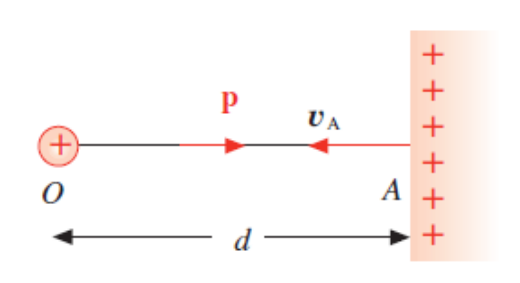
\includegraphics[scale=0.3]{e_2_5.png}
\subsubsection*{Formule utilizzate}

\subsubsection*{Soluzione}
$V(B) - V(A) = \left(\frac{q}{4\pi\epsilon_0 \frac{d}{4}} - \frac{q}{4\pi\epsilon_0 d}\right) + \left(-\frac{\sigma}{2\epsilon_0}\frac{3d}{4}-0\right) = \frac{3}{4\pi\epsilon_0 d}\left(q - \frac{\pi}{2}\sigma d^2\right) = 52.47\ V$
\\$E_k(B) = E_k(A)-e[V(A) - V(B)] = \frac{1}{2}m_eV_A^2 + e[V(B) -V(A)]$
\\$V_B = \sqrt{\frac{2E_k(B)}{m_e}} = 5.24 * 10^6\frac{m}{s}$
\newpage

\end{document}